
%-----------------------------  README  ------------------------------------------
% THESIS TEMPLATE FILE - compatible with University of Leeds guidelines, and designed
% for use when submitting an alternative format thesis / thesis by publication.
% Key point is that by using biber instead of bibtex, bibliographies for each publication
% can be created from a single .bib file.
%
% Instructions:
%   - Tested to work on Overleaf (as of July 2020)
%   - Otherwise to compile yourself:
%     pdflatex 0_thesis.tex
%     biber 0_thesis                                            % NOTE NO EXTENSION FOR BIBER!
%.    makeindex 0_thesis.nlo -s nomencl.ist -o 0_thsis.nls      %Only needed if using the nomencl package for nomenclature
%     pdflatex thesis.tex
%
% Installing / getting it to compile:
%    When used with TexLive on Ubuntu 18.04, some other packages and biber are needed:
%    e.g. in a terminal:
%     sudo apt install texlive-bibtex-extra                                            % Usually missing if breakcites.sty can't be found
%     sudo apt install biber                                                           % used instead of biblatex as it supports refsections (which allows a bibliography in each chapter from a single .bib file)

%    Others that may be needed:
%      sudo apt-get install texlive-fonts-extra
%
%     Errors from missing .sty files are usually to do with missing packages.
%
% Latexdiff:
%    Great for tracking changes.  A nice guide to what can be a tricky install is here:
%    http://www.deanbodenham.com/learn/troubleshooting-latexdiff.html


% History
%     M.C.   Garthwaite 30/09/2011
%     D.P.S. Bekaert 	23/02/2016  Adapt for thesis by publication
%     M.E. 	 Gaddes		13/03/2019	Adapt to handle references from a single .bib file
%     M.E.   Gaddes     05/06/2020  Create minimum working template
%.    S.M.   Greenwood  17/06/2020  Re-adapted for traditional thesis submission, tidied up preamble, and tested on Overleaf.

%-----------------------------------------------------------------------




\documentclass[titlepage,twoside,onecolumn,a4paper,11pt]{report}

\edef\restoreparindent{\parindent=\the\parindent\relax}
\usepackage{parskip}
\restoreparindent

\usepackage{float}
\usepackage{fancyhdr} 								% for making headers and footers
\usepackage{appendix} 								% sets up the appendix environment
\usepackage{graphicx} 								% Needed to display graphics
\usepackage{geometry}                               % Allows definition of text/page measurements
\usepackage{setspace} 								% \singlespacing , \onehalfspacing , and  \doublespacing
\usepackage{url} 									% line-breaks for long URLs, DOIs, etc
\usepackage{amsmath}                                % AMS mathematics
\usepackage{amssymb}                                % Defines names of maths symbols in amsfonts
\usepackage{a4}                                     % for A4 paper size. Not needed if defined in \documentclass ?
\usepackage{enumerate}                              % useful for customising lists
\usepackage{bm}                                     % Allows bold math symbols with e.g. \bm{\tau}
\usepackage{array}                                  % Used for fixing size of columns/rows in tables
\usepackage{multirow}                               % Used for joining specific cells of tables together


\usepackage{nomencl}                                % for the Nomenclature
\makenomenclature                                   % Tells latex to expect a nomenclature so create the relevant auxiliary file

\usepackage{etoolbox}                               % Creates groupings for the nomenclature list.
\renewcommand\nomgroup[1]{                          % If you don't want this just comment these lines of code out
  \item[\bfseries                                   % and make sure you don't give an argument when adding to the nomenclature
  \ifstrequal{#1}{A}{Acronyms}{                 % later on (i.e \nomenclature{t}{time} instead of \nomenclature[S]{t}{time}
  \ifstrequal{#1}{U}{Units and Prefixes}{       % You can remove or add groups as you please.
  \ifstrequal{#1}{N}{Mathematical Notation}{    %
  \ifstrequal{#1}{S}{Symbols}{}}}}              %
]}                                                  %


\DeclareUnicodeCharacter{2032}{$^\prime$}           %Declare the 'prime' unicode character so latex knows what to do with it if it encounters it. I encountered this issue due to a reference containing the prime character which gave an error since it wasn't in math mode
%\DeclareUnicodeCharacter{0301}{*************************************}      # Might have to deal with this one as well.


\usepackage[small,bf]{caption}                      % Sets the style of the captions for figure/table. here the text
\usepackage[left,mathlines]{lineno}                 % Places line numebrs in margin
\usepackage[nottoc,notbib]{tocbibind}               % Puts List of Figures, the List of Tables, the Bibliography and the Index all to be added to the Table of Contents
\usepackage[pdftex,pdfpagelabels,breaklinks=true]{hyperref}  % Creates hyper links N.B. pdf option and index option [pdftex,hyperindex,backref,pdfpagelabels]
\usepackage[all]{hypcap}                            % Hyperlinks go to all of figure rather than just caption. Problem if figure does not have a caption - Conflicts with {fltpage}
\usepackage[normal]{subfigure}                      % allows multiple floats within one figure environment with a caption for each in addition to main caption
\usepackage{breakcites}                             % Makes a minor change to \cite to make sure it behaves properly with multiple citations

\usepackage{makeidx}                                % Make Index
\makeindex                                          % Tells latex to make the relevant auxiliary file    
\usepackage{lipsum} % Purely to print some lorem ipsum dummy text in this template. Not needed for the actual thesis.

% I either chose to not use these packages or they were already commented out when I came to use the previous version of this template
% I'll leave them here incase they are of use in the future

%\usepackage{breakurl}
%\usepackage{doi}  % Need to download sty file. Add doi links N.B. must go after hyperref. Also it won't work with doi's with < >. For % put \%. doi links are only compatible with certain bib style files



%%%%%%%%%%%%%%%%%%%% Bibliography stuff. Argh!!!!
%\usepackage[backend=biber, style=apa, natbib=true, citestyle=authoryear, uniquename=false, maxcitenames=1]{biblatex}		          %
\usepackage[backend=biber,
            natbib=true,                                % using natbib allows the use of citet and citep, so you can copy from JGR file
            citestyle=authoryear,                       %
            bibstyle=authoryear,                        % no number of bibliography
            maxcitenames=2,                             % switch to firsname + et al if more than 2
            maxbibnames=99,                             % don't truncate authors to et al in bibliography
            uniquename=false,                           % control inititals and get correct number of authors (no name1, name2, et al)
            uniquelist=false,                           % ditto
            doi=false,                                  % Remove unwanted fields from bibliography
            isbn=false,
            url=false,
            eprint=false
            ]{biblatex}

\addbibresource{references.bib}                        % include extension for biber
%%%%%%%%%%%%%%%%%%%% End Bibliography stuff.



%%%% Pdf name etc setup
\hypersetup{
    plainpages=false,                   % Resets counter in main matter (Problems of links to early pages)
    bookmarks=true,                     % show bookmarks bar?
    unicode=false,                      % non-Latin characters in Acrobat\u2019s bookmarks
    pdftoolbar=true,                    % show Acrobat\u2019s toolbar?
    pdfmenubar=true,                    % show Acrobat\u2019s menu?
    pdffitwindow=true,                  % page fit to window when opened
    pdfstartview={FitV},
    pdftitle={Simulations of the thermo-chemical evolution of the Earth’s core with stable stratification.},    % title
    pdfauthor={Sam Greenwood},          % author
    pdfcreator={School of Earth and Environment, University of Leeds},
    pdfsubject={PhD Thesis, School of Earth and Environment, University of Leeds},   % subject of the document
    pdfkeywords={},
    pdfdisplaydoctitle=true,
    % SET up LINKS
    colorlinks=true,% false: boxed links; true: colored links
    citecolor=black,% color of links to bibliography
    filecolor=black,% color of file links
    linkcolor=black,% color of internal links
    urlcolor=black  % color of external links
}





%%%% Page setup
\pagestyle{fancy}                                   % 'fancy' will place header and footers. 'plain' will not
\renewcommand{\chaptermark}[1]{\markboth{\chaptername\ \thechapter:\ #1}{}} % sets format of Chapter mark (left pages)
\renewcommand{\sectionmark}[1]{\markright{\S\thesection\ #1}} % sets format of section mark (right pages)
\renewcommand{\headrulewidth}{0.5pt}                % sets thickness of header rule
\renewcommand{\footrulewidth}{0pt}                  % sets thickness of footer rule
\fancyhead[RO,LE]{\thepage} 						% options R - Right-hand side L - Left-hand side O - odd page E - even page
% \fancyhead[RE]{\nouppercase\leftmark}
% \fancyhead[LO]{\nouppercase\rightmark}
\fancyfoot{}
%\setlength\headheight{13.6pt}					% if paper titles stay on one page in the headers
\setlength\headheight{26.0pt}					% if paper titles go onto two pages in the headers
\fancyhfoffset[EL,OR]{0mm}
\onehalfspacing
%\doublespacing						 % alternative \onehalfspacing. both acceptable for Leeds submissions
%\geometry{a4paper,twoside,inner=40mm,outer=25mm,top=30mm,bottom=35mm}		% Definition of page measurements compatible with University of Leeds margin requirements (40mm x 20mm x 20mm x 20mm).
\geometry{a4paper,inner=40mm,outer=25mm,top=30mm,bottom=35mm}				% Larger margin for binding side
%%%% End page setup

%%%%%%%%%%%%%%%%%%%%%%%%%%%%%%%%%%%%%%%%%%%%%%%%%%%%%%%%%%%%%%%%%%%%%%%%%%%%%%%%%%%%%%%%%%%% End Preamble %%%%%%%%%%%%%%%%%%%%%%%%%%%%%%%%%%%%%%%%%%%%%%%%%%%%%%%%%%%%%%%%%%%%%%%%%%%%%%%%%%%%%%%%%%%%
\begin{document}
\pagenumbering{roman}                                           % Start roman numbering, to be used up until introduction.

\makeatletter
\def\cleardoublepage{\clearpage\if@twoside \ifodd\c@page\else%
\hbox{}%
\thispagestyle{empty}
\newpage%
\if@twocolumn\hbox{}\newpage\fi\fi\fi}
\makeatother

%%%%%%%%%%%%%%%%%%%%%%%%%%%% Title Page %%%%%%%%%%%%%%%%%%%%%%%%%%%%
\title{
\huge{\textbf{An impressive sounding thesis title}}\\[2cm]
\Large{{\bf Sam Greenwood}} \\[4cm]
\large{Submitted in accordance with the requirements for the degree of\\
Doctor of Philosophy} \\[2cm]
\large{The University of Leeds}\\
\large{School of Earth and Environment}\\ [2cm]
\large{July 2020} }
\author{} \date{}
\pdfbookmark[0]{Title page}{Title page} % Sets a PDF bookmark for the title page
\maketitle
\cleardoublepage

%%%%%%%%%%%%%%%%%%%%%%%%%%%% Declaration %%%%%%%%%%%%%%%%%%%%%%%%%%%%
% \fancyhead[RE,LO]{Declaration}						% text, right edge of even pages, left edge of odd
% \fancyhead[RO,LE]{\thepage}							% page number, right edge of odd pages, left of even
The candidate confirms that the work submitted is their own and that appropriate credit has been given where reference has been made to the work of others.\\

This copy has been supplied on the understanding that it is copyright material and that no quotation from the thesis may be published without proper acknowledgement\\

Copyright \copyright\; 2020 The University of Leeds and Sam Greenwood\\
The right of Sam Greenwood to be identified as Author of this work has been asserted by him in accordance with the Copyright, Designs and Patents Act 1988.
\cleardoublepage

%Change author names in copyrights ^


%%%%%%%%%%%%%%%%%%%%%%%%%%%% Acknowledgments %%%%%%%%%%%%%%%%%%%%%%%%%%%%
\chapter*{Acknowledgements}
\fancyhead[RE,LO]{Acknowledgements}
\fancyhead[RO,LE]{\thepage}

I'd like to thank Stackoverflow for contributing the majority of my code, and to Wikipedia for always explaining topics that university lectures never could. I'd also like to thank Wolframalpha for solving my equations and fo never telling anyone that I couldn't integrate $\sqrt{x}$.

\cleardoublepage

\newcommand {\dd} {\mathrm{d}}
\newcommand {\DD} {\mathrm{D}}
\newcommand {\dpar} {\partial}
\newcommand{\dS}{\cdot \mathrm{d}\mathbf{S}}
%
\newcommand{\Vs}{V_{\mathrm{s}}}
\newcommand{\Voc}{V_\mathbf{2}}
\newcommand{\Vconv}{V_\mathbf{2}}
\newcommand{\Mconv}{M_\mathbf{2}}
\newcommand{\Vis}{V_\mathbf{12}}
\newcommand{\Vsl}{V_\mathbf{3}}


\newcommand{\Mc}{M_{\mathrm{c}}}
\newcommand{\Moc}{M_{\mathrm{oc}}}
\newcommand{\Mic}{M_{\mathrm{ic}}}
\newcommand{\ri}{r_{\mathrm{i}}}
\newcommand{\rc}{r_{\mathrm{c}}}
\newcommand{\rs}{r_{\mathrm{s}}}
\newcommand{\Tcen}{T_{\mathrm{cen}}}
\newcommand{\Tc}{T_{\mathrm{c}}}
\newcommand{\Ti}{T_{\mathrm{i}}}
\newcommand{\Ts}{T_{\mathrm{s}}}
\newcommand{\Ta}{T_{\mathrm{a}}}
\newcommand{\Tm}{T_{\mathrm{m}}}
\newcommand{\dr}{\Delta \rho}
\newcommand{\rhoi}{\rho_{\mathrm{i}}}


\newcommand{\TFe}{T_{\mathrm{m, Fe}}}
\newcommand{\dTX}{\Delta T_{\mathrm{x}}}
\newcommand{\SFe}{\Delta s_{\mathrm{Fe}}}
\newcommand{\lams}{\lambda_X^s}
\newcommand{\laml}{\lambda_X^l}


\newcommand{\ca}{c_\mathbf{2}}
\newcommand{\cs}{c_x^s}
\newcommand{\cl}{c_x^l}
\newcommand{\cbars}{\bar{c}_x^s}
\newcommand{\cbarl}{\bar{c}_x^l}
\newcommand{\alphad}{\alpha_\mathrm{D}}

\newcommand{\Qg}{Q_{\mathrm{g}}}
\newcommand{\Qh}{Q_{\mathrm{H}}}
\newcommand{\Qs}{Q_{\mathrm{s}}}
\newcommand{\Qr}{Q_{\mathrm{r}}}
\newcommand{\Qupper}{Q^-_{\mathrm{r_s}}}
\newcommand{\Qlower}{Q^+_{\mathrm{r_s}}}
\newcommand{\Qa}{Q_{\mathrm{a}}}
\newcommand{\Ql}{Q_{\mathrm{l}}}
\newcommand{\Qp}{Q_{\mathrm{P}}}
\newcommand{\Q}{Q_{\mathrm{c}}}

\newcommand{\Eg}{E_{\mathrm{g}}}
\newcommand{\Eh}{E_{\mathrm{H}}}
\newcommand{\Es}{E_{\mathrm{s}}}
\newcommand{\Ek}{E_{\mathrm{k}}}
\newcommand{\Er}{E_{\mathrm{r}}}
\newcommand{\El}{E_{\mathrm{L}}}
\newcommand{\Ep}{E_{\mathrm{P}}}
\newcommand{\Ej}{E_{\mathrm{J}}}
\newcommand{\Ea}{E_{\alpha}}

%
\newcommand{\massf}{\mathbf{i}}
\newcommand{\q}{\mathbf{q}}
\newcommand{\n}{\hat{\mathbf{n}}}
\newcommand{\uvel}{\mathbf{u}}
\newcommand{\vel}{\mathbf{v}}
\newcommand{\B}{\mathbf{B}}
\newcommand{\E}{\mathbf{E}}
\newcommand{\z}{\mathbf{z}}

\newcommand{\BV}{Brunt-V{\"a}is{\"a}l{\"a} }
%%%%%%%%%%%%%%%%%%%%%%%%%%%% Abstract %%%%%%%%%%%%%%%%%%%%%%%%%%%%
\chapter*{Abstract}
\fancyhead[RE,LO]{Abstract}
\fancyhead[RO,LE]{\thepage}

There are currently some observations in this specific area of science, which are important because presumably somebody cares. Previous authors tried to explain them with some data/maths but I think they did so incompletely. Here I include more data/maths because it wasn't complicated enough already and I can't get a PhD if I don't. I perform some kind of experimental procedure and some kind of modelling technique that my supervisor told me to use to show that these observations can indeed be explained by something. My 4 years of work therefore demonstrates that previous authors were out by 1\%, within the range of uncertainty.


\cleardoublepage



%%%%%%%%%%%%%%%%%%%%%%%%%%%% Contents page %%%%%%%%%%%%%%%%%%%%%%%%%%%%
\pdfbookmark[0]{Contents}{Contents}
\fancyhead[RE,LO]{Contents}
\fancyhead[RO,LE]{\thepage}
\tableofcontents
\cleardoublepage

%%%%%%%%%%%%%%%%%%%%%%%%%%%% Lis of figures %%%%%%%%%%%%%%%%%%%%%%%%%%%%
\fancyhead[RE,LO]{List of Figures}
\fancyhead[RO,LE]{\thepage}
\listoffigures
\cleardoublepage

%%%%%%%%%%%%%%%%%%%%%%%%%%%% Nomenclature %%%%%%%%%%%%%%%%%%%%%%%%%%%%
%You don't have to define these here, you can define them throughout the document as they appear if you wish
%I personally think its neat to have the definitions separate and not scattered throughout the thesis.

\nomenclature[A]{CMB}{Core Mantle Boundary}
\nomenclature[A]{BRB}{Be Right Back}


\nomenclature[N]{$\oint$}{Surface integral}
\nomenclature[N]{$\nabla$}{Gradient}
\nomenclature[N]{$\nabla\cdot$}{Divergence}
\nomenclature[N]{$\mathcal{O}(x)$}{Order of magnitude of $x$}
\nomenclature[N]{$\sum{}$}{Summation}

\nomenclature[S]{$\gamma$}{Gr{\"u}neisen parameter}
\nomenclature[S]{$\eta$}{Magnetic diffusivity}


\nomenclature[U]{eV}{Electron volt}
\nomenclature[U]{G}{Giga, $1\times10^9$}


\printnomenclature

\cleardoublepage
\fancyhead[RE]{\leftmark}		% Return Headers to Normal
\fancyhead[LO]{\rightmark}




\pagenumbering{arabic}           % Switch to normal numbers, also resets counter
\chapter[Introduction]{Introduction}  %[Chapter name as it will appear in the ToC]{chapter name as it will apear as the title to the chapter} Probably always want them to be the same 
\label{ch:introduction}

\section{Overview}

This thesis is about someting.


\section{Equations}

An example of an equation (solve it for bonus points)

\begin{equation}
     x = 35A + \frac{3B}{100},
\end{equation} where typically $A$ and $B$ are taken as 12 and 23 respectively.

We can align equations 
\begin{align}
    \frac{\partial y}{\partial x} &= 3x^2 \\
    y(0) &= 0.\\
\end{align}

Sometimes we have such a long equation that we need to split is across 2 lines. We can choose to withhold numbering both lines since it's all one equation

\begin{align}
    \overbrace{\int k\left(\frac{\nabla T}{T}\right)^2\dd V}^{\Ek}
    &+ \overbrace{\int\frac{\massf^2}{\alphad T}\dd V}^{\Ea}
    + \overbrace{\int\frac{\Phi}{T} \dd V}^{\Ej} = \nonumber\\
    & \overbrace{-\int\left(\frac{1}{\Tc}-\frac{1}{T}\right)\rho C_p\frac{\DD T}{\DD t}\dd V}^{\Es}
    + \overbrace{\left(\frac{1}{\Tc}-\frac{1}{\Ti}\right)\Ql}^{\El}
    + \overbrace{\frac{\Qg}{\Tc}}^{\Eg}.
\label{eq:entropy budget final}
\end{align}This was my most complicated equation and I include it here to inflate my ego.

In equation \ref{eq:entropy budget final} I have made use of using symbols that I frequently use defined in the symbols.tex file. dd, DD, Ek, Ej, Es, El, Eg, massf, Tc, and Ti are all defined in symbols.tex. If it's not worth it to you to have any predifined symbols then you can simply delete symbols.tex and remove the `include symbols.tex' from the preamble.
\cleardoublepage % dump remaining floats before end of chapter and ensure the next chapter starts on odd (right-hand) side
\fancyhead[RE]{\leftmark}
\fancyhead[LO]{\rightmark}


\chapter[Including Figures]{Including Figures}
\label{ch:chapter2}


\section{Introduction}

Chapter 1 introduced including equations. In this chapter I will show how figures are included


\section{Figures}

Here is a figure. A useful way to define the width of the figure is by some fraction of the textwidth. Depending on how much white space is around the figure you'll have to play around with this to get it to the size you want it.

\begin{figure}[!hbt]
    \centering
    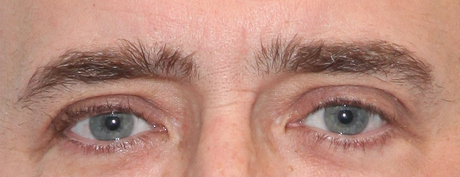
\includegraphics[width=0.8\textwidth]{chapter2_figures/GuessWho.jpg}
    \caption{Can you guess whose eyes these belong to?}
    \label{fig:guess who}
\end{figure}

%\clearpage
\section{Common issues}

Placement of figures is really the only difficulty you'll likely encounter. Often \LaTeX will end up placing the figure too far below where you want it, or even in the next section.

\begin{figure}[!hbt]
    \centering
    
\includegraphics[width=0.9\textwidth]{chapter2_figures/code.png}
    \caption{Not sure that programming would be feasible without copy/paste}
    \label{fig:code}
\end{figure}

In Fig. \ref{fig:code}, the [!hbt] options specified after `begin figure' tell \LaTeX where to try to place the figure in order. First try placing here as specified in the tex file (h), otherwise try at the bottom of the page (b), otherwise try placing at the top of the page (t). The exclamation point specified to overrule any behaviour for figure placement that \LaTeX may have (e.g. from the document class I think?).

Sometimes the figure will end up in the next section, not what we want! As a last resort I will add the clearpage just before the next section forcing placement of figures/tables before the new section starts. You might end up with some extra white space but it's a compromise sometimes we have to make.


\begin{figure}[!hbt]
    \centering
    
\includegraphics[width=\textwidth]{chapter2_figures/yesbutno.png}
    \caption{By the time we come to write up, we've all been asked this at least once. This is the honest answer.}
    \label{fig:yes but no}
\end{figure}

%\clearpage
\section{Next section}

Here's some \textit{Lorem ipsum} to bulk out the text and show that the figure is being placed in this section, despite being part of the previous section. Uncommenting the clearpage command just above the section command will force the figure to be placed, then clear the page before coming to this section.

Fun fact, \textit{Lorem ipsum} is typically a corrupted version of \textit{De finibus bonorum et malorum}, a first-century BC text by the Roman statesman and philosopher Cicero, with words altered, added, and removed to make it nonsensical, improper Latin (according to Wikipedia anyway). It is used as placeholder text since the word length distribution is about the same as English and so serves as a useful representation of what text will end up looking like (in terms of number of words on a line etc).

\lipsum[1-2]
\cleardoublepage % dump remaining floats before end of chapter and ensure the next chapter starts on odd (right-hand) side
\fancyhead[RE]{\leftmark}
\fancyhead[LO]{\rightmark}


\chapter[Another chapter]{Another chapter}
\label{ch:chapter3}

\section{Introduction}

Not really much more to say tbh. Afraid you need to just get on with it now.

\section{Methods}

\section{Results}

\section{Discussion and Conclusions}
\cleardoublepage % dump remaining floats before end of chapter and ensure the next chapter starts on odd (right-hand) side
\fancyhead[RE]{\leftmark}
\fancyhead[LO]{\rightmark}


\chapter[A further chapter]{A further chapter}
\label{ch:chapter4}

\section{Introduction}

Again, just get on with it.

\section{Methods}

\section{Results}

\section{Discussion and Conclusions}
\cleardoublepage % dump remaining floats before end of chapter and ensure the next chapter starts on odd (right-hand) side
\fancyhead[RE]{\leftmark}
\fancyhead[LO]{\rightmark}


\chapter[The final chapter]{The final chapter}
\label{ch:conclusions_futurework}

Oh, one last thing I guess are references. You can cite papers with the (author, year) e.g. This effect is significant \citep{Davies2015}. or just the year e.g. The study of \citet{Mound2019RegionalVariations} found ...

I personally wrote this thesis in Overleaf and linked it to my mendeley account to directly import the bib file. I liked to just copy the paper title and paste into Mendeley's desktop app `Literature search', then drop that paper into my `Thesis' group. Sync on the app, then refresh the file on Overleaf and it's done. Do whatever works for you best.

A note on using Overleaf. They will only compile your document if it takes less than 1 minute (4 minutes for the pro account). Once you start including lots of figures, for a thesis, you will easily exceed 1 minute limit. You could start downloading the source files and compiling them locally but that's probably a faff. There's lots of information out there on using desktop apps with \LaTeX. I was lucky to have had a v1 Overleaf account, that when transferred to the new v2 account, kept the git integration that is now a paid feature. I could just git pull to my local drive then compile with the included Makefile (even make local changes and push those back to Overleaf if I didn't have an internet connection). I did this just because I was used to the Overleaf editor and quite liked it but, as always, do whatever works best for you.

All the best with finishing your PhD. It will be long, hard, and uncomfortable at times (that's what she said?) and nobody finds it easy, you are not alone. It will feel like you've learnt more about your project in the 6 months of writing than you did in the preceding 3 years. Never worry about creating a perfect (or even decent for that matter) draft of your thesis, best to get chapters off to your supervisors for comments earlier rather than later. Even the version you submit will still need to have whatever changes the examiners suggest applied. I submitted yesterday and as I put together this template, I've already found a mistake. A thesis is never finished, just submitted.
\cleardoublepage % dump remaining floats before end of chapter and ensure the next chapter starts on odd (right-hand) side
\fancyhead[RE]{\leftmark}
\fancyhead[LO]{\rightmark}

\cleardoublepage
\printbibliography[heading=bibintoc]

\chapter*{Appendix}
\addcontentsline{toc}{chapter}{Appendix} 

Put all the work that really should have featured in the main document but you didn't have the time/space here.
\cleardoublepage % dump remaining floats before end of chapter and ensure the next chapter starts on odd (right-hand) side
\fancyhead[RE,LO]{Appendix A}
\fancyhead[RO,LE]{\thepage}


\end{document}
